\documentclass[12pt,a4paper]{article}
\usepackage[utf8]{inputenc}
\usepackage[spanish,es-tabla]{babel}
\usepackage{amsmath}
\usepackage{amsfonts}
\usepackage{amssymb,latexsym,cancel}
\usepackage{graphicx}
\usepackage[left=2cm,right=2cm,top=2cm,bottom=2cm]{geometry}
\renewcommand{\baselinestretch}{1.5}
\usepackage{epstopdf}
\usepackage{subfigure}
\usepackage{array}
\usepackage{float}
\usepackage{longtable}
\newcolumntype{E}{>{$}c<{$}}
%%%%%%%%%%%%%%%%%%%%%%%%%%%
\usepackage{fancyhdr}
\pagestyle{fancy}
\fancyhead{}
\fancyhead[R]{ }
\fancyfoot[C]{\thepage}
\renewcommand{\headrulewidth}{0.9pt}
\renewcommand{\footrulewidth}{0.9pt}
\usepackage{url}


\begin{document}


\title{Actividad 2\\ Introducción a python, jupyter y pandas  }
\author{
 Jorge Benz Olguín Aguilar\\
\small{División de Ciencias Exactas, Departamento de Física}\\
\small{Universidad de Sonora}\\
}
\date{\small{\today}}
\maketitle

\section{Introducción}

Jupyter es una herramienta ideal para todo aquel que desea aprender a programar con python y necesiten ir documentando todo lo que van aprendiendo, además de aquellos que deben presentar informes con bases científicas.

Esta aplicación web de codigoabierto, desarrollada utilizando lenguaje HTML que permite crear, compartir y editar documentos en los que se puede ejecutar código python, hacer anotaciones, insertar ecuaciones, visualizar resultados y documentar funcionalidades. Esta aplicación está diseñada para tener una compatibilidad avanzada con python e incluye la posibilidad de exportar documentos hechos con la herramienta a otros formatos.

generalmente está herramienta es utilizada para la enseñanza del lenguaje de programación python, la limpieza y transformación de datos científicos, la simulación numerica, el modelado estadistico y muchas otras áreas.

\begin{enumerate}

\item De fácil instalación gracias a estar presente en la Suite Anaconda Distribution.

\item Posee una avanzada interfaz web que permite combinar código fuente, textos, formulas, figuras y multimedia en un solo documento.

\item La integración de diverso tipos de información nos permite dar explicaciones más adecuada de nuestros programas o de los conceptos que estemos aprendiendo.

\item Permite el acceso desde cualquier lugar sin necesidad de instalación de otros servicios, ya que funciona como cliente servidor. De igual manera, Se puede ejecutar en un escritorio local o en servidor remoto.

\item Aunque el lenguaje de programación fundamental en Jupyter Notebook es Python, esta aplicación también es compatible con más de 40 lenguajes, entre los que destacan R, Julia y Scala.

\item Permite el intercambio de documentos de Jupyter a través de servicios de terceros.

\item Podemos ejecutar y visualizar imágenes, videos, LaTeX y JavaScript, además de manipular los resultados de los mismos en tiempo real.

\item Cuenta con un administrador de documentos avanzado, que permite visualizar los archivos compatible con Jupyter Notebook que esten alojados en nuestro equipo.

\item Los documentos realizados en Jupyter Notebook se pueden exportar a diferentes formatos estáticos incluyendo HTML, reStructeredText, LaTeX, PDF y presentaciones de diapositivas.

\item Es compatible con nbviewer el cual permite que portar nuestros documentos de Jupyter Notebook a la nube como una página web estática, la cuál podrá ser visualizada por cualquiera sin necesidad de instalar el Jupyter Notebook .

\end{enumerate}


Las tres primeras son gáficas del ejemplo.ipynb, variación de la rapidez de los vientos, gráfica de temperatura y humedad relativa y variación de la temperatura.


\begin{figure}[H]
  \centering
  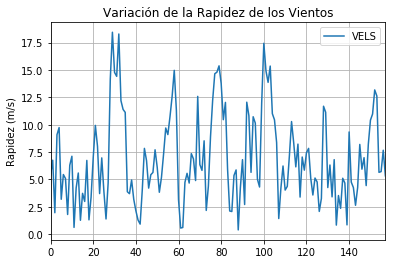
\includegraphics[scale=0.7]{velocidad_viento.png}
  \caption{Rapidez del Viento}
  \label{fig:RapV}
\end{figure}


El comportamiento de la humedad y y la temperatura queda por demas desnudado por la gráfica, se observa claramente que cuando la temeperatura es muy alta la humedad relativa disminuye.


\begin{figure}[H]
  \centering
  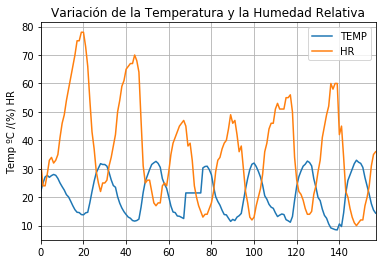
\includegraphics[scale=0.7]{temp_hr.png}
  \caption{Temperatura y humedad relativa}
  \label{fig:TemyHum}
\end{figure}



\begin{figure}[H]
  \centering
  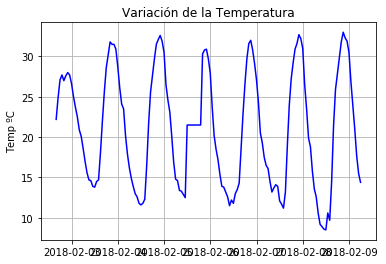
\includegraphics[scale=0.7]{temp.png}
  \caption{Temperatura}
  \label{fig:Tem}
\end{figure}

Las siguientes gráficas corresponden a los datos obtenidos del http://smn1.conagua.gob.mx/emas/  , especificamente los datos de Bahía Kino. Dentro de los datos encontramos mediciones de velocidad de los vientos, rapidez de las rafagas de viento, radiación solar, humedad relativa, dirección de los vientos entre otras.
\\

En la siguiente gráfica podemos observar como las rafagas de viento se incrementan hacia la tarde-noche.

\begin{figure}[H]
  \centering
  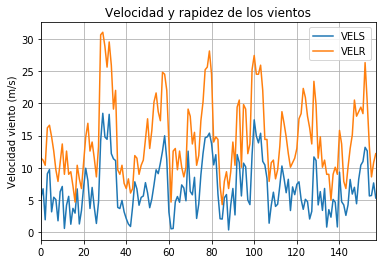
\includegraphics[scale=0.7]{velrap_vientos.png}
  \caption{Velocidad del viento y Rafagas}
  \label{fig:VyR}
\end{figure}



\begin{figure}[H]
  \centering
  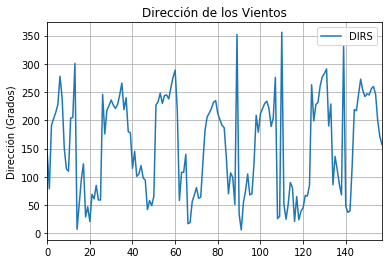
\includegraphics[scale=0.7]{dir_viento.png}
  \caption{Dirección del Viento}
  \label{fig:DirVie}
\end{figure}

La radiación solar como es de esperarse es más alta entre las doce del medio día y las cinco de la tarde.

\begin{figure}[H]
  \centering
  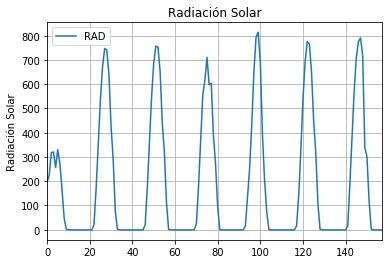
\includegraphics[scale=0.5]{rad_sol.png}
  \caption{Radiación Solar}
  \label{fig:rad_sol}
\end{figure}


\subsection{Apéndice}

\begin{enumerate}
\item ¿Cúal es tu primera impresión de Jupyter Notebook?
R. Tiene una imagen muy agradable, da la impresión que es una especie de ipython mejorado, bueno, al menos en la presentación. No estoy en condiciones para realizar una comparación mas profunda sobre las capacidades de cada cual. Parece muy bueno para manejar datos, la visualización de tablas y gráficos es muy buena. Lo que podría criticar sería el hecho de que cuando tenga un codigo largo va a ser un poco complicado volver y mejorarlo.

\item ¿Se te dificulto leer codigo en python?
R. El codigo en python es muy entendible, muy limpio si vale la expresión, por lo que resulta un poco mas facil de entender que fortran, por mencionar uno que mas o menos conozco. Lo cierto es que programar requiere de muchas horas, tiene una curva de aprendizaje muy tendida, por lo quq necesita de mucho trabajo y paciencia.

\item ¿En base a tu experiencia de programación en fortran, que te parece el entorno de trabajar en python?
R. Mucho pero mucho mejor, cualquiera que quiera empezar en el mundo de la programación debería empezar por python. No tengo mucho tiempo trabajando con python, pero por lo que he escuchado es un lenguaje que se lleva muy bien con el analisis de datos.

\item A diferencia de Fortran, ahora se producen las gráficas utilizando la biblioteca Matplotlib. ¿Cómo fue tu experiencia?.
R: La biblioteca de matplotlib es muy buena, podemos realizar gráficas de una forma facil. El tener que utilizar programas externos a fortran para poder graficar datos resultaba en proceso bastante frustrante. En python solo tenemos que importar la biblioteca y listo, aprevechemos sus capacidades.

\item En general, ¿qué te pereció el entorno de trabajo en Python?
R. Como dije antes, el trabajar con python ha resultado en una experiencia muy agradable, espero poder aprender mucho mas de python.

\item ¿Qué opinas de la actividad? ¿Estuvo compleja? ¿Mucho material nuevo? ¿Que le faltó o que le sobró? ¿Qué modificarías para mejorar? La practica como tal fue buena. El material si que fue bastante, aunque es de suponerse que el material se ira trabajando poco a poco durante todo el curso.

\end{enumerate}





\begin{thebibliography}{0}


\bibitem {desdelinux}https://blog.desdelinux.net/jupyter-notebook/

\end{thebibliography}

\end{document}